This section describes the specific tools used in the experiments. It starts with presenting the deployed Kubernetes cluster's layout. Then, the tools needed to run the actual experiments are introduced. Finally, this section concludes with a brief overview of the three test applications used

\subsection{Kubernetes cluster}
\label{cluster}
All the experiments are run on a Kubernetes cluster deployed on the DistriNet private cloud, which is based on the OpenStask platform \citep{openstack}. Four virtual machines are deployed: one master and three worker nodes. The cluster itself is created using \textit{kubeadm} \citep{kubeadm}. All of the machines are running the Ubuntu 16.04 operating system. Three of the nodes, including the master node, are allocated 2 CPUs and 4 GB of memory. The last node is assigned 4 CPUs and 8 GB of memory. The three worker nodes are placed on the same OpenStack computing node to minimize latencies between applications running on the nodes. On the first worker node, which is the node with 4 CPUs and 8GB of memory, an experiment controller is deployed. The second and third worker nodes are reserved for the applications to be deployed on. An overview of the setup is shown in Figure \ref{fig:cluster}.

\setlength\abovecaptionskip{3pt}
\begin{figure}[h]
\centering
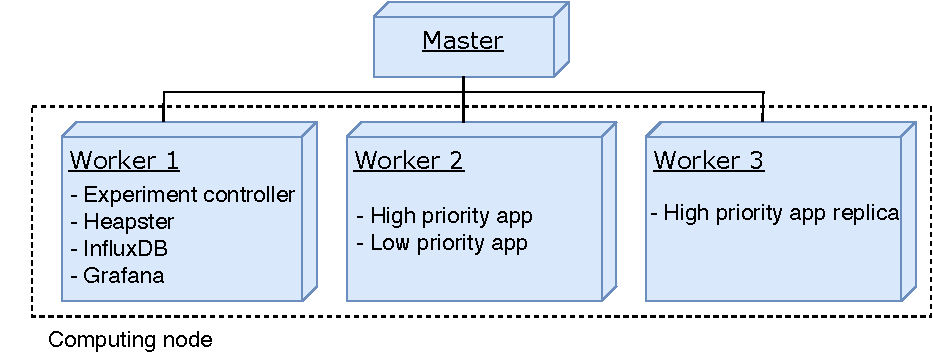
\includegraphics[width=0.75\textwidth]{Images/Setup/Cluster.pdf}
\caption{Cluster setup}
\label{fig:cluster} 
\end{figure}


\subsection{Experimentation tools}
\label{tools}

Running the experiments requires various tools to send a customizable load to the test applications, as well as to monitor the application's performance and the resource usage of all the nodes and pods. 

\subsubsection{Resource monitoring}
To monitor the resources in the cluster, a combination of Heapster \citep{heapster}, InfluxDB \citep{influxdb} and Grafana \citep{grafana} is employed. Heapster collects each node's metrics through Kubelet, which is the primary Kubernetes node agent running on each worker node \citep{kubelet}\citep{heapster-influxdb-grafana}. The collected data is written to InfluxDB. InfluxDB is a time-series database, a database optimized for time-stamped or time series data \citep{timeseriesdb}. Grafana is a metric dashboard and graph editor which supports, among others, InfluxDB \citep{grafana-github}. 

\subsubsection{Experiment controller}
To run and monitor the experiments, K8-Scalar \citep{scalar} is used. K8-Scalar is an ``extensible workbench exemplar for implementing and evaluating different self-adaptive approaches to autoscaling container-orchestrated services'' \citep{scalar-github-overview}. K8-Scalar can be customized to test a specific system by implementing Java user and request classes fit for that system. Multiple users may be implemented, for example one user which performs CPU-intensive requests and one which performs memory-intensive requests. \\

When preparing an experiment, the distribution of the types of users can be specified, for example 95\% of the users executing memory intensive requests and 5\% executing CPU intensive requests. Furthermore, the exact workload profile can be described using a template, part of which is shown in listing \ref{listing:profile}. An experiment in K8-Scalar consists of multiple runs, and the peak load for each of these runs must be provided. A run in turn consists of a ramp-up phase, a peak load phase and a ramp-down phase. The duration of all of these phases can be configured. In between runs, there can also be constant low load phases. Ramping up and down is done linearly. Besides sending the requests, K8-Scalar monitors the time needed by the tested applications to process these requests \citep{scalar}.

\lstset{caption={Load profile example},label=listing:profile}
\begin{lstlisting}[float,floatplacement=H]
## LOAD PROFILE
# The number of concurrent users for peak load for the entire cluster. 
# For each number in this comma separated list, a new run is started.
user_peak_load=500,1000,1500
user_warmup_fraction=1
user_warmup_duration=0
user_ramp_up_duration=0
user_peak_duration=400
user_ramp_down_duration=0
user_cooldown_duration=0
user_wait_inbetween_runs=0
\end{lstlisting}

\newpage

\subsection{Deployed applications}
\label{test-apps}

\subsubsection{LMaaS: Log Management as a Service}
In accordance with the K8-Scalar paper \citep{scalar}, a Log Management-as-a-Service (LMaaS) application based on Cassandra is selected as the first high priority application with which to evaluate the Kubernetes mechanics in a CPU intensive environment. The main service offered by the application is real-time aggregation and storage of log files. Only write operations are examined in this thesis, as they are CPU intensive. The main QoS requirement for the application is thus the latency of write requests. Cassandra well-suited as for the experiments as its design is optimized for write-heavy workloads. \citep{scalar}.

\subsubsection{Artificial SaaS application}
\label{setup:saas-app}
A second high priority application is also experimented with to to verify whether the experimental results are valid for more than just one application. An artificial SaaS application developed at KU Leuven \citep{saas-app} is selected for this purpose. The main benefit of this SaaS application is that the stressed resource is easily configurable through the application's REST interface. For example, if a CPU intensive workload needs to be tested, the memory intensity of the application can be set to zero by executing a simple REST command at runtime. 

\subsubsection{Low priority application}
\label{setup:lpp}
The application shown in Figure \ref{fig:cpu-app-python} is deployed as the low priority application when testing the effects of co-locating pods. It uses up CPU cycles by constantly executing a multiplication. If sufficient resources are free, this application continually uses one full CPU since it is single threaded. The main benefit of this application is that its exact CPU usage is known and roughly constant.
\newpage

\bigskip
\begin{figure}[htbp]
\centering
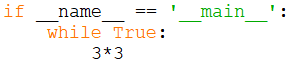
\includegraphics[width=0.45\textwidth]{Images/Experiments/Cpu-app.PNG}
\caption{Low priority application Python code}
\label{fig:cpu-app-python}
\end{figure}
\null
\vfill
